\section{Robot Hardware}
\label{sec:robot_hardware}

\subsection{Torsional Spring Leg}
\label{sec:torsional_spring_leg}

Figure \ref{fig:assembly_CAD} shows the CAD model for the torsional spring leg design, including both knee and hip extension/flexion motor, as well as the hip adduction/abduction motor. The CAD model was created using the CAD software Solidworks. An annotated exploded view of the leg can be seen in figure \ref{fig:CAD_leg_exploded_annotate}, while an annotated exploded view for the hip motor housing can be seen in figure \ref{fig:exploded_motor_housing_hip}. 

Components planned for in-house manufacturing are shown in figure \ref{fig:manufacture_only} The axle that will be 
threaded and screwed directly into the motor shaft, and lead directly into a ball bearing, is emphasized in red. The leg is designed for aluminum manufacturing due to aluminum's high strength-to-weight ratio and machinability. While 3D-printable plastics are lighter, aluminum's superior strength allows for a lighter overall design when accounting for the required structural integrity \cite{Aluminum} \cite{PLA}, barring complications from manufacturing.

\begin{figure}[h!]
    \centering
    \begin{subfigure}[b]{0.45\textwidth}
        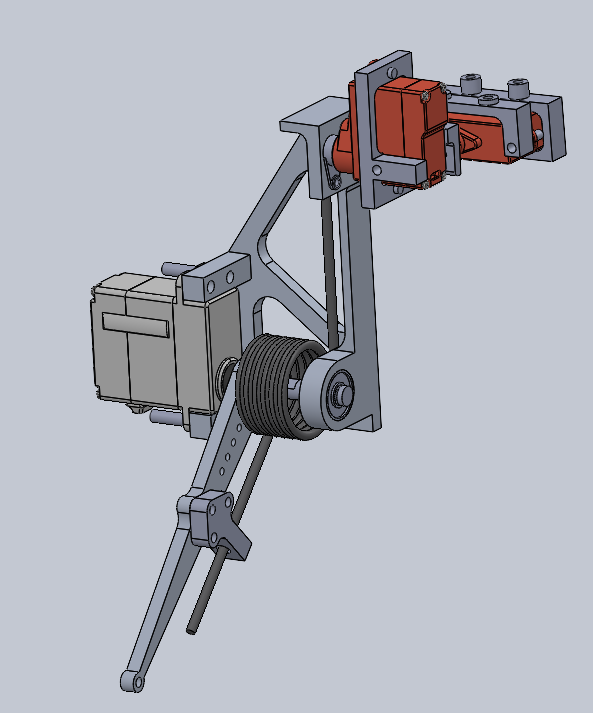
\includegraphics[width=\textwidth]{Images/CAD_leg_inside_bent.png}
        \caption{The bearing supporting the knee-joint shaft reduces off-axis loads on the motor shaft.}
        \label{fig:image1}
    \end{subfigure}
    \hfill
    \begin{subfigure}[b]{0.45\textwidth}
        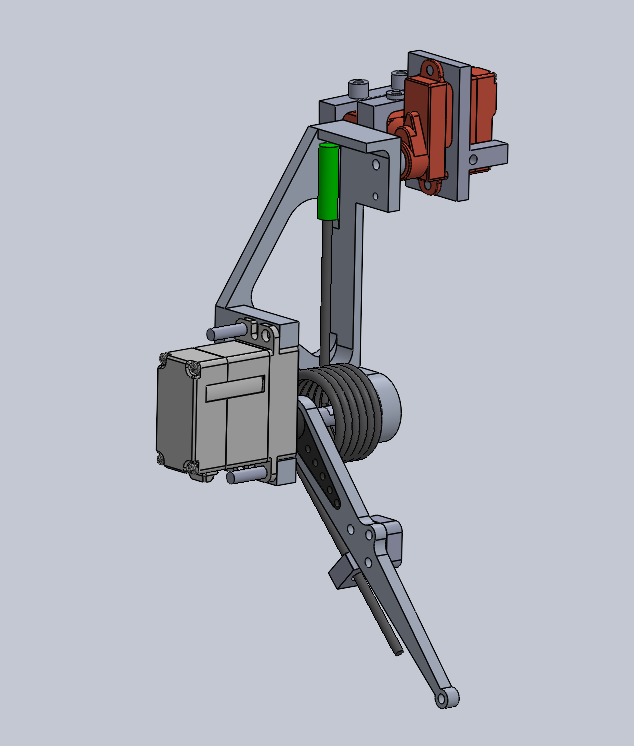
\includegraphics[width=\textwidth]{Images/CAD_leg_outside_bent.png}
        \caption{A green plastic (PLA) holster reduces friction at the spring-leg contact point.}
        \label{fig:image2}
    \end{subfigure}
    \caption{Torsional spring leg CAD model.}
    \label{fig:assembly_CAD}
\end{figure}

\begin{figure}[h!]
    \centering
    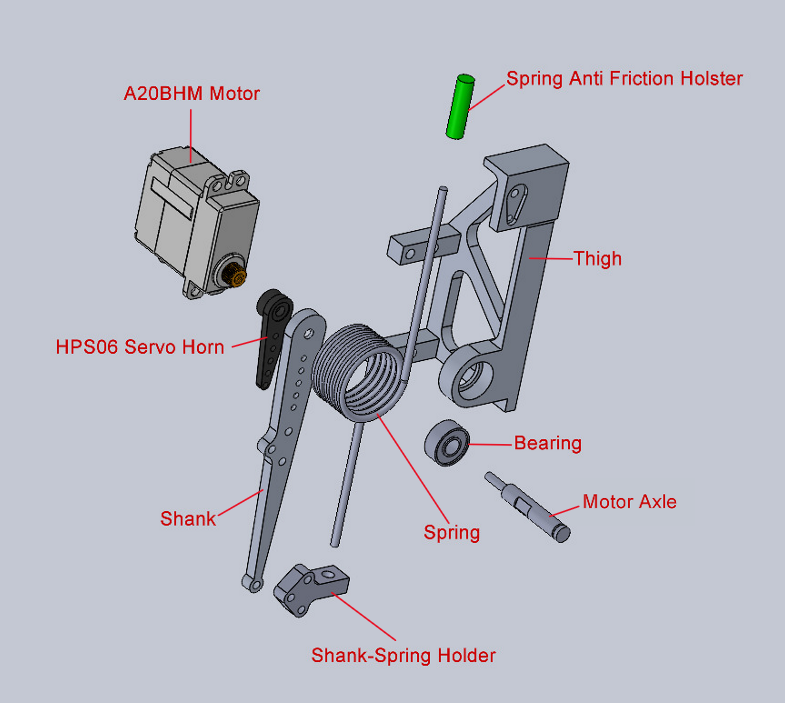
\includegraphics[width=0.6\textwidth]{Images/CAD_leg_exploded_annotate.png}
    \caption{Annotated exploded view of the CAD leg design.}
    \label{fig:CAD_leg_exploded_annotate}
\end{figure}

\begin{figure}[h!]
    \centering
    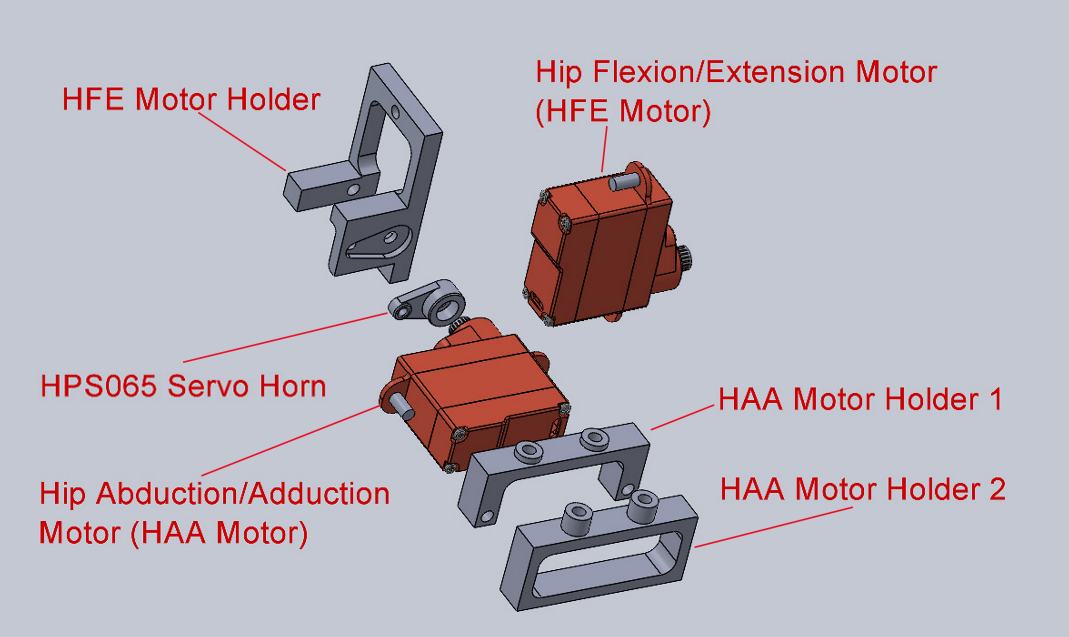
\includegraphics[width=0.6\textwidth]{Images/exploded_motor_holder_hip.png}
    \caption{Exploded view of the hip joint motor housings.}
    \label{fig:exploded_motor_housing_hip}
\end{figure}

\begin{figure}[h!]
    \centering
    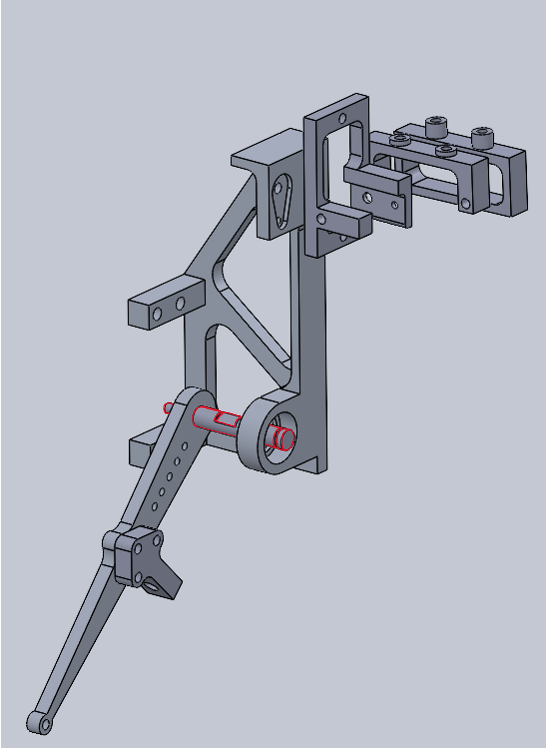
\includegraphics[width=0.6\textwidth]{Images/manufacture_only2.png}
    \caption{CAD model of components for in-house manufacture, with the motor shaft axle highlighted in red, which will lead directly into a ball bearing.}
    \label{fig:manufacture_only}
\end{figure}

Initial load testing of a 3D printed thigh prototype with the spring (figure \ref{fig:printed_leg_and_spring}) indicates sufficient strength for spring compression, suggesting 3D printing may be viable for the leg structure. The motor shaft axle will still be manufactured in aluminum.

\begin{figure}[h!]
    \centering
    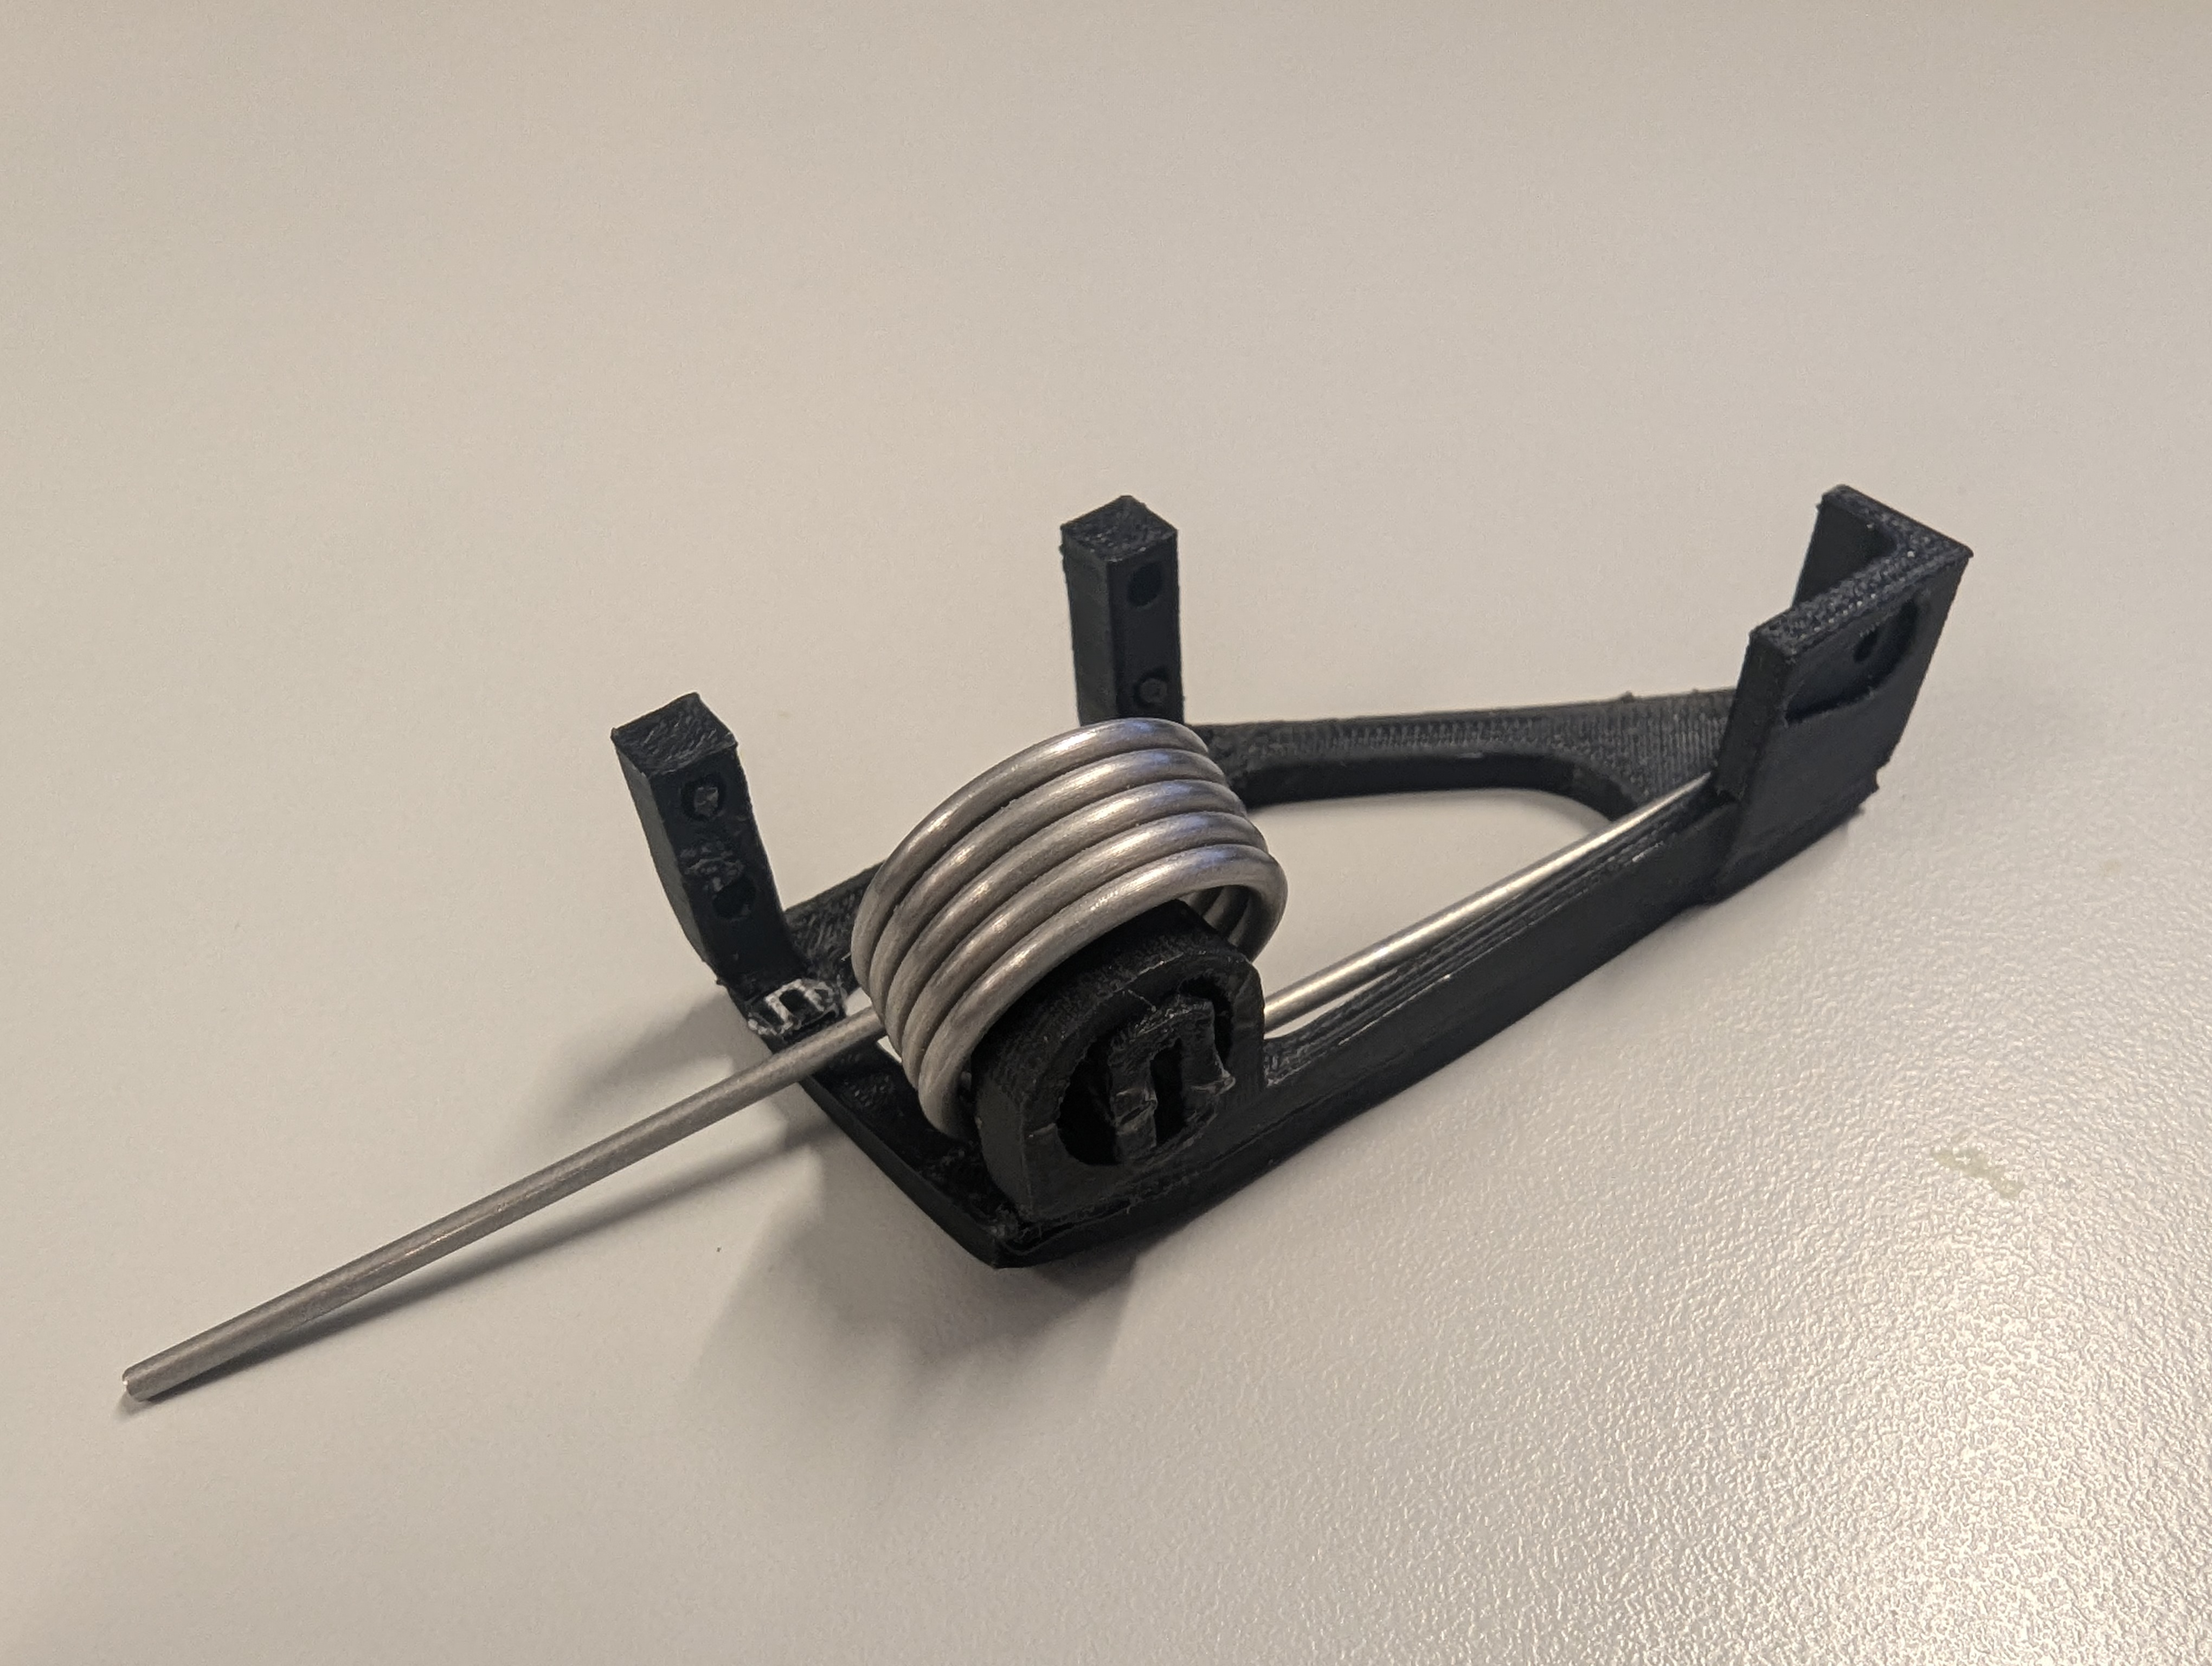
\includegraphics[width=0.6\textwidth]{Images/printed_leg_and_spring.jpg}
    \caption{3D printed thigh prototype with torsional spring.}
    \label{fig:printed_leg_and_spring}
\end{figure}

\subsection{Extension Spring Leg Design}
\label{sec:extension_spring_design}

The extension spring design (figure \ref{fig:extension_spring_CAD}) was abandoned due to spring-shank collision at full knee flexion (-180 degrees). Avoiding this collision by moving the spring attachment point inward toward the body such that the spring could lie parallel to the leg would create an unacceptable moment arm on the motor shaft.

\begin{figure}[h!]
    \centering
    \begin{subfigure}[b]{0.45\textwidth}
        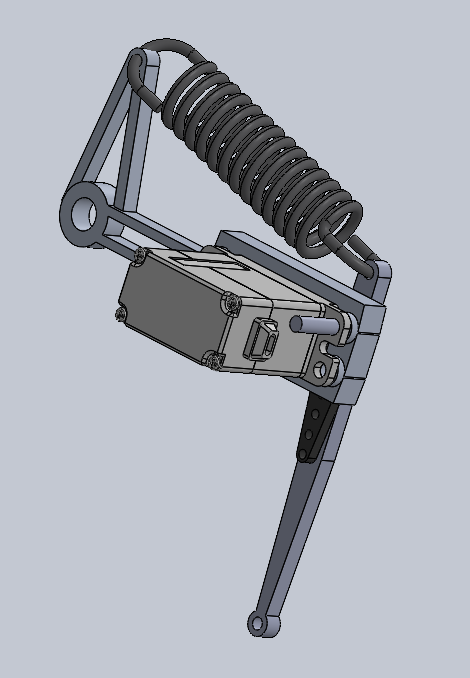
\includegraphics[width=\textwidth]{Images/extension_spring_outside.png}
        \label{fig:extension_spring_outside}
    \end{subfigure}
    \hfill
    \begin{subfigure}[b]{0.45\textwidth}
        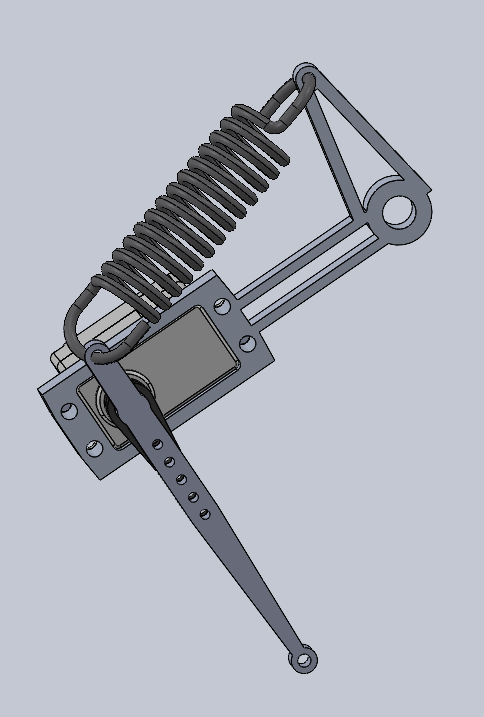
\includegraphics[width=\textwidth]{Images/extension_spring_inside.png}
        \label{fig:extension_spring_inside}
    \end{subfigure}
    \caption{Extension spring configurations: outside (left) and inside (right) the leg.}
    \label{fig:extension_spring_CAD}
\end{figure}

\subsection{Motor Selection}
\label{sec:motor_selection}

AGF-RC motors were selected for their superior torque-to-weight ratio. Table \ref{tab:motor_selection} lists the specific motors chosen, with detailed specifications in appendices \ref{appendix:A06CLS_V2_website_information} to \ref{appendix:A20_info}.

\begin{table}[h!]
    \centering
    \begin{tabular}{|c|c|}
        \hline
        Joint & Motor\\ \hline
        Knee flexion/extension & A20BHM \\
        Hip flexion/extension & A06CLS V2 \\
        Hip adduction/abduction & A06CLS V2 \\ \hline
    \end{tabular}
    \caption{Selected Motors}
    \label{tab:motor_selection}
\end{table}

The A20BHM was chosen over the heavier A35CHM (specifications in appendix \ref{appendix:A35CHM_motor_info}) which offers only marginally higher torque. We were unable to find other motors in a similar weight class that could provide comparable torque and speed. The A06CLS V2 selection reasoning is detailed in section \ref{sec:hip_motor_dimensioning_test_design}.

The physical thigh design is heavier than its simulation counterpart, which is simplified to a rectangular prism, due to additional width needed for motor and spring integration. However, this mass difference is negligible compared to the motor and body masses. Table \ref{tab:thigh_mass_comparison} compares thigh masses for different materials.

\begin{table}[h!]
    \centering
    \begin{tabular}{|c|c|c|}
        \hline
        Material Density & Simulation Thigh Mass & Actual Design Mass \\ \hline
        1200 kg/m\textsuperscript{3} (Tough PLA) \ref{appendix:tough_PLA} & N/A & 6.45 g \\
        2700 kg/m\textsuperscript{3} (Aluminum 6061) & 2.26 g & 14.27 g \\
        \hline
    \end{tabular}
    \caption{Thigh mass comparison between simulation and actual design for different materials (calculated using Solidworks Mass Properties).}
    \label{tab:thigh_mass_comparison}
\end{table}

\subsection{Other Purchased Components}

Table \ref{tab:other_purchased_components} lists additional required components, excluding standard screws and nuts.

\begin{table}[h!]
    \centering
    \begin{tabular}{|c|c|c|}
        \hline
        Component & Name/Part Number & Supplier \\ \hline
        Bearing & RS: 612-5802 &  RS \\
        Left leg spring &  T075-180-484L & Sodemann\\
        Right leg spring &  T075-180-484R & Sodemann\\
        Knee servo horn & HPS06 & AGF-RC\\
        Hip servo horns & HPS065 & AGF-RC\\
        \hline
    \end{tabular}
    \caption{Additional purchased components.}
    \label{tab:other_purchased_components}  
\end{table}